% 2010 安徽理 19题 图1 : 同 2010 安徽文 17 题图, 另标注角平分线 l
\usetikzlibrary{arrows.meta,calc}
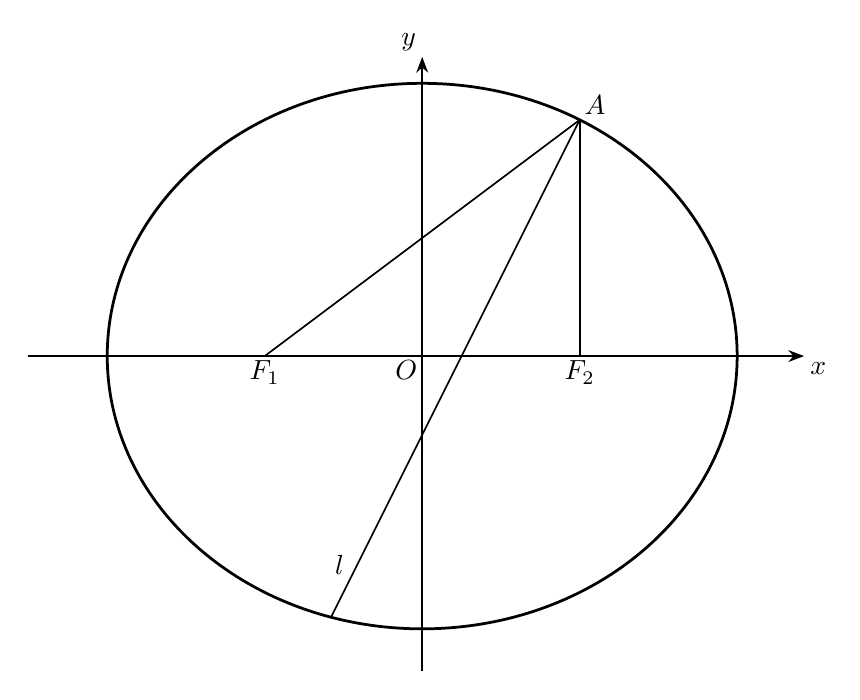
\begin{tikzpicture}[x=1cm,y=1cm,font=\normalsize,line width=.6pt,>=Stealth]
\draw[->] (-5,0)--(4.85,0) node[below right,inner sep=2pt] {$x$};
\draw[->] (0,-4)--(0,3.8) node[above left,inner sep=2pt] {$y$};
\node[below left,inner sep=1.5pt] at (0,0) {$O$};
\draw[line width=1pt] (0,0) ellipse [x radius=4.0, y radius=3.464102];
\coordinate (A) at (2,3);
\coordinate (F1) at (-2,0);
\coordinate (F2) at (2,0);
\coordinate (Q) at (-1.157895,-3.315789);
\draw (A)--(F1);
\draw (A)--(F2);
\draw (A)--(Q);
\node[above right,inner sep=1.5pt] at (A) {$A$};
\node[below,inner sep=1.5pt] at (F1) {$F_1$};
\node[below,inner sep=1.5pt] at (F2) {$F_2$};
\node at (-1.05,-2.65) {$l$};
\end{tikzpicture}
